\Needspace{12\baselineskip}
\originalchapter{NMR量子信息的五道公开预习题}
本章题面来自Junior Lab的\texttt{exp49}手册第一页，五题确实公开，不能归入其他手册所指向的不可取得课前网页。解答为编者独立推导；新程序逐矩阵核验脉冲、oracle及单侧FID，未声称在实体NMR仪器完成实验。以下基顺序始终为 $|HC\rangle=|00\rangle,|01\rangle,|10\rangle,|11\rangle$，质子H在左、碳C在右。手册门公式还使用“第一量子bit写在右”的编号约定，故本章用H/C与张量因子代替容易混淆的1/2下标。

\originalsection{人口差与实际谱读出}
\begin{exercise}
（原预习题1）对角密度矩阵 $\rho=\operatorname{diag}(a,b,c,d)$ 作用 $R_x(\pi/2)$ 读出脉冲后，两个质子峰的积分为 $a-c,b-d$，两个碳峰为 $a-b,c-d$。(a)画出a、b、c、d各自单独非零的四种谱；(b)求手册热态的峰积分；(c)对热态作用真正CNOT或near-CNOT后，求所得谱并比较。手册近似热态为 $I/4+10^{-4}\operatorname{diag}(5,3,-3,-5)$。
\end{exercise}
\begin{solution}
读出脉冲把纵向人口差变为横向磁化，两个不同邻核态给两条允许单自旋跃迁线。若只一个人口为1，其余为0，峰积分按固定的两条质子线、两条碳线顺序为
\[
\begin{array}{c|rrrr}
\rho&H_1&H_2&C_1&C_2\\\hline
|00\rangle\langle00|&1&0&1&0\\
|01\rangle\langle01|&0&1&-1&0\\
|10\rangle\langle10|&-1&0&0&1\\
|11\rangle\langle11|&0&-1&0&-1
\end{array}
\]
\begin{center}
\begin{tikzpicture}[x=.85cm,y=.75cm]
\foreach \row/\state/\a/\b/\c/\d in {0/00/1/0/1/0,1/01/0/1/-1/0,2/10/-1/0/0/1,3/11/0/-1/0/-1}{
 \begin{scope}[yshift=-\row*2.2cm]
 \node[left] at (-.3,0) {$|\state\rangle$};
 \draw[->] (0,0)--(2.8,0) node[right] {H};
 \draw[->] (4,0)--(6.8,0) node[right] {C};
 \draw[main,very thick] (.8,0)--(.8,\a);\draw[main,very thick] (1.8,0)--(1.8,\b);
 \draw[blue,very thick] (4.8,0)--(4.8,\c);\draw[blue,very thick] (5.8,0)--(5.8,\d);
 \fill[main] (.8,\a) circle(1pt);\fill[main] (1.8,\b) circle(1pt);
 \fill[blue] (4.8,\c) circle(1pt);\fill[blue] (5.8,\d) circle(1pt);
 \end{scope}}
\end{tikzpicture}
\end{center}
图中每根谱线的正负高度表示上表的\emph{积分}，同种核的两频率相隔J；横轴只示意核种内频率，不把H与C绝对频率画在同一尺度。真实有限线宽可用后文Lorentzian替换每根线，面积符号保持不变。

正负表示同一接收相位约定下的吸收峰方向，未出现的线积分为0；图形只需把对应频率的峰按这些符号和相对面积画出，不能把人口本身当峰面积。恒等矩阵部分在所有人口差中消去。

以 $\epsilon=10^{-4}$ 记热态偏离，$a=1/4+5\epsilon,b=1/4+3\epsilon,c=1/4-3\epsilon,d=1/4-5\epsilon$，故质子两峰均为 $8\epsilon$，碳两峰均为 $2\epsilon$。H/C的约4倍Larmor频率比造成这个高温人口差比例。它是手册的高温近似幅度，不是本项目测得的谱强。

左H控制、右C目标的CNOT交换 $|10\rangle,|11\rangle$，因此人口变为 $(a,b,d,c)$，谱为 $(10\epsilon,6\epsilon,2\epsilon,-2\epsilon)$。near-CNOT在同一置换上附带基态相位，对角热态的相位在 $U\rho U^\dagger$ 中消去，所以两种门在这一次热态人口谱中相同。检验真正量子门不能止于四个经典输入输出或对角态；必须用相干输入、相位敏感读出或过程重构揭示相对相位。

有J耦合时，每种核的两峰相距J，峰中心是各自旋转框架参考的Larmor位置。实验先测H、C谱中心与分裂、标定90度脉宽和接收相位，再按积分或拟合面积比较上表。基线、重叠线宽及相位错误能改变表观正负，不应只从最大谱高直接判断人口差。
\end{solution}

\originalsection{Pauli指数与旋转角}
\begin{exercise}
（原预习题2）显式计算 $U=\exp[\ii(n_x\sigma_x+n_y\sigma_y+n_z\sigma_z)]$，证明 $U=I\cos|\mathbf n|+\ii(\mathbf n\cdot\boldsymbol\sigma)\sin|\mathbf n|/|\mathbf n|$。
\end{exercise}
\begin{solution}
Pauli关系为 $\sigma_i\sigma_j=\delta_{ij}I+\ii\epsilon_{ijk}\sigma_k$。对实向量n，反对称项与 $n_in_j$ 相乘后求和为0，故 $(\mathbf n\cdot\boldsymbol\sigma)^2=|\mathbf n|^2I$。指数的偶次项为I乘余弦，奇次项为 $\ii(\mathbf n\cdot\boldsymbol\sigma)/|\mathbf n|$ 乘正弦，得到所求式；n为0时按连续极限取I。

本章实际旋转采用 $R_\alpha(\theta)=\exp(-\ii\theta\sigma_\alpha/2)$，因此题目正号指数对应绕n方向角 $-2|\mathbf n|$ 的旋转。区分指数向量长度与Bloch球转角，可避免把90度脉冲误写成指数中90度。程序以一般非轴向n检验矩阵指数，残差低于 $10^{-12}$。
\end{solution}

\originalsection{CNOT的完整相位校正脉冲}
\begin{exercise}
（原预习题3）从手册near-CNOT出发，给出矩阵非零元均为1的真正受控非门，只允许无关的整体相位。至多再用四个x/y轴旋转，或两个z轴旋转完成校正；给出脉冲顺序。
\end{exercise}
\begin{solution}
弱耦合、共振旋转框架的耦合Hamiltonian为
\[H_J=2\pi\hbar JI_z^HI_z^C=(\pi\hbar J/2)Z_HZ_C.\]
自由演化 $\tau=1/(2J)$ 给 $U_J=\exp[-\ii\pi Z_HZ_C/4]$。按算符从右先作用的约定，手册的near门写为
\[
 U_{\rm near}=R_y^C(-\pi/2)U_JR_x^C(\pi/2)
 =\e^{\ii\pi/4}\begin{pmatrix}
 -\ii&0&0&0\\0&1&0&0\\0&0&0&-\ii\\0&0&-1&0
 \end{pmatrix}.
\]
它的经典置换正确，但 $|00\rangle,|01\rangle,|10\rangle,|11\rangle$ 带不同相位，不能只删除一个整体相位就称为CNOT。

两个z校正须放在正确的一侧：
\[
 U_{\rm near}R_z^H(\pi/2)R_z^C(-\pi/2)
 =\e^{-\ii\pi/4}\begin{pmatrix}
 1&0&0&0\\0&1&0&0\\0&0&0&1\\0&0&1&0
 \end{pmatrix}.
\]
所以时间顺序为：先H的 $z$轴 $+\pi/2$ 与C的 $z$轴 $-\pi/2$ 校正，再C的 $x$轴 $+\pi/2$，等待 $1/(2J)$，最后C的 $y$轴 $-\pi/2$。两核z旋转彼此可交换，但不能任意把目标核的校正移到near门另一侧。

若仅能直接做x/y旋转，利用 $R_z(\theta)=R_x(-\pi/2)R_y(-\theta)R_x(\pi/2)$，并合并相邻目标核旋转，得到同一门的时间顺序：H依次 $x:+\pi/2,y:-\pi/2,x:-\pi/2$；C依次 $x:+\pi/2,y:+\pi/2$；等待 $1/(2J)$；C最后 $y:-\pi/2$。这是在原near序列之外至多四个额外x/y旋转的实现。独立NumPy计算两序列到目标矩阵的误差均低于 $10^{-12}$，保留完整复相位核验而不只比较概率。

上述理想脉冲忽略硬脉冲期间的J演化，要求脉宽相对 $J^{-1}$ 足够短，两个参考频率和相位已校准。失谐与不同核 $B_1$ 不均匀会产生误差；必要的refocusing须把残余Zeeman演化与所需J演化分开设计。软件矩阵通过并不等于硬件门的保真度已测出。
\end{solution}

\originalsection{四个oracle与Deutsch--Jozsa矩阵}
\begin{exercise}
（原预习题4）列出一位输入、一位输出的四个经典函数，画对应经典和量子逻辑关系。量子oracle应保持x并将y变为 $y\oplus f(x)$。给出仅用x/y旋转和J自由演化延迟的四条脉冲序列；计算原手册 $U_k=R_{\bar y}^H R_y^C U_{f_k}R_y^H R_{\bar y}^C$ 的四乘四矩阵，所有单核旋转角为 $\pi/2$。
\end{exercise}
\begin{solution}
函数为常数0、常数1、身份x和反相 $1-x$。经典电路分别给常数0/1、直通、NOT；可逆量子oracle分别为 $I_4,I_H\otimes X_C,\mathrm{CNOT}_{H\to C},(I_H\otimes X_C)\mathrm{CNOT}_{H\to C}$。加入y作异或目标后，即使f为常数也不丢弃输入信息。

四个经典真值关系为
\[
\begin{array}{c|rrrr}x&f_0&f_1&f_x&f_{1-x}\\\hline
0&0&1&0&1\\1&0&1&1&0\end{array}.
\]
以下量子电路保留x，目标输出为 $y\oplus f(x)$；实心控制要求x为1，空心控制要求x为0。
\begin{center}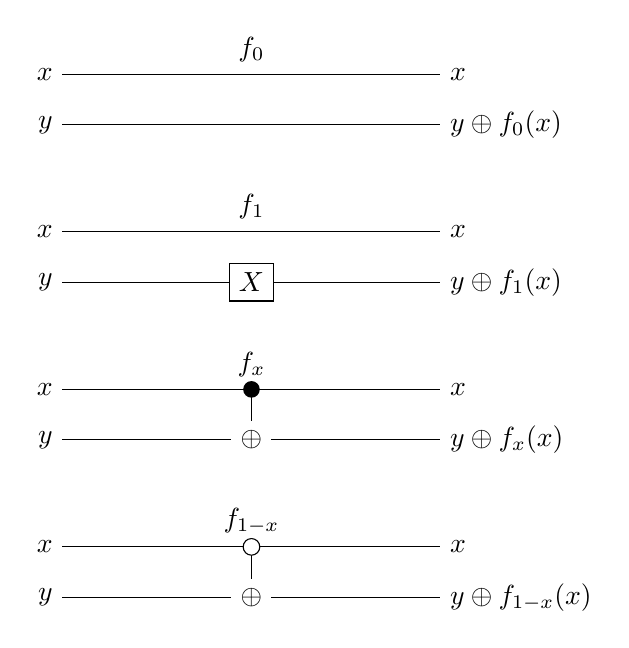
\begin{tikzpicture}[x=.8cm,y=.8cm]
\foreach \r/\name in {0/f_0,1/f_1,2/f_x,3/f_{1-x}}{
\begin{scope}[yshift=-\r*2cm]
\node[left] at (0,0) {$x$};\node[left] at (0,-.8) {$y$};
\draw (0,0)--(6,0) node[right] {$x$};\draw (0,-.8)--(6,-.8) node[right] {$y\oplus\name(x)$};
\node[above] at (3,.05) {$\name$};
\end{scope}}
\node[draw,fill=white] at (3,-3.3) {$X$};
\draw (3,-5)--(3,-5.8);\fill (3,-5) circle(3pt);\node[fill=white] at (3,-5.8) {$\oplus$};
\draw (3,-7.5)--(3,-8.3);\draw[fill=white] (3,-7.5) circle(3pt);\node[fill=white] at (3,-8.3) {$\oplus$};
\end{tikzpicture}\end{center}
用上题已校正的CNOT脉冲S，四序列为“不加门”、C的 $R_x(\pi)$、S、S后再加C的 $R_x(\pi)$。每个S含明确的J延迟 $1/(2J)$，其余单核脉冲需按各核90度标定宽度加倍或改相位。$R_x(\pi)=-\ii X$ 只增加整体相位。若限定x/y，可将S中的z校正全部改成上题已核验的x/y顺序，而无需借用未给的第三方门库。

写 $A=R_y^H(\pi/2)R_y^C(-\pi/2)$，$B=R_y^H(-\pi/2)R_y^C(\pi/2)$，则 $U_k=BU_{f_k}A$。统一舍去每个完整电路的整体相位，四矩阵为
\[
 U_0=I_4,\qquad U_1=\operatorname{diag}(-1,1,-1,1),
\]
\[
 U_x=\begin{pmatrix}0&0&-1&0\\0&1&0&0\\-1&0&0&0\\0&0&0&1\end{pmatrix},\qquad
 U_{1-x}=\begin{pmatrix}0&0&1&0\\0&1&0&0\\1&0&0&0\\0&0&0&1\end{pmatrix}.
\]
因此输入 $|00\rangle$，两个常函数输出H为0，两个平衡函数输出H为1；C返回0。相对符号由oracle相位回传到控制核，未调用f两次。用经典热混合态直接读取则仍需人口差解释，不能把纯态电路的确定性结论直接改写为所有热态核均处于同一输出。

原手册采用时间标记来提取拟纯态信号：通过几次人口置换保持00人口不变、轮换另三个人口，再平均谱，可使另三个人口平均相同。线性NMR读出看不到恒等矩阵部分，剩下的偏离矩阵按 $|00\rangle$ 的算法演化产生信号；这不是把整份高熵样品物理净化成纯态。实际算法报告应保存各次原始谱、平均权重和相位，不只给一条看似纯态的最终线。
\end{solution}

\originalsection{单侧FID与吸收、色散线形}
\begin{exercise}
（原预习题5）计算 $s(t)=\e^{\ii(\omega_0t+\phi)}\e^{-t/T_2}$ 从0到 $+\infty$ 的单侧Fourier变换，并联系原手册Lorentzian的中心、宽度和相位参数。
\end{exercise}
\begin{solution}
采用 $\widetilde s(\omega)=\int_0^\infty s(t)\e^{-\ii\omega t}\dd t$，$T_2>0$ 时
\[
 \widetilde s(\omega)=\frac{\e^{\ii\phi}}{T_2^{-1}+\ii(\omega-\omega_0)}.
\]
记 $\alpha=T_2^{-1},\Delta\omega=\omega-\omega_0$，实部为 $[\alpha\cos\phi+\Delta\omega\sin\phi]/(\alpha^2+\Delta\omega^2)$。接收相位为0时是对称吸收Lorentzian；相位偏离会混入反对称色散部分，不能把它当作新增峰或人口变化。吸收线的半高全宽为 $2/T_2$弧度每秒，即 $1/(\pi T_2)$Hz，中心为 $\omega_0$，整体幅度取决于人口差及接收增益。

实际记录有限时长 $t_m$ 时，还乘 $1-\e^{-(\alpha+\ii\Delta\omega)t_m}$；离散采样、窗和静场分布改变线形。自由感应衰减的表观宽度常反映 $T_2^*$，不自动等于回波得到的真正 $T_2$。程序对一个明确参数组以复积分核对解析变换，未生成假装来自NMR仪器的真实FID。
\end{solution}
